\section{Background on \eqsat}
\label{sec:back}

\begin{figure}[t]
\footnotesize
  \begin{minipage}{0.55\linewidth}
    \begin{lstlisting}[xleftmargin=0pt]
    def equality_saturation($t$, $R$):
      egraph = empty_egraph()
      $c_{\sf root}$ = egraph.add($t$)                       $\label{ln:eqsat-init}$
      saturated = False
      until saturated or timeout():
        saturated = True
        for $\ell \rewritesto r$ in $R$:
          for ($\sigma$, $c_\ell$) in egraph.search($\ell$): $\label{ln:eqsat-ematch}$
            $c_r$ = egraph.add($\sigma(r)$)                  $\label{ln:eqsat-add}$
            if not egraph.same_eclass($c_\ell$, $c_r$):
              egraph.union($c_\ell$, $c_r$)                  $\label{ln:eqsat-merge}$
              saturated = False
      return egraph.extract_best($c_{\sf root}$)             $\label{ln:eqsat-extract}$
  \end{lstlisting}
  \end{minipage}
  \begin{minipage}{0.44\linewidth}
    \begin{center}
    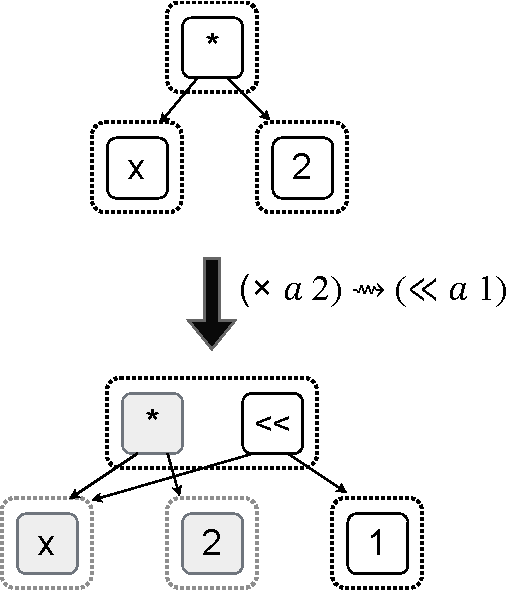
\includegraphics[scale=0.5]{fig/background.pdf}
    \end{center}
  \end{minipage}
  \caption{
    (Left) The \eqsat algorithm~\citep{eqsat, egg, ruler}. Initially, a
    new \egraph is created that represents the input term $t$.
    Sound rewrite rules
    are applied until saturation or some resource bound (like iteration limit
    or timeout) is reached.
    A cost function is used to extract the ``best'' program from the
    \egraph.
    (Right) Examples of two \egraphs before and after applying
    the rewrite $(\times ~ a ~ 2) \rewritesto (\ll ~ a ~ 1)$.
    The dotted boxes represent \eclasses and the solid boxes represent \enodes.
    The \egraph on top represents the
    AST (abstract syntax tree) of the input term,
    $(\times ~ x ~ 2)$, and the \egraph below
    shows that the \eclasses that represent the terms $(\times ~ x ~ 2)$ and
    $(\ll ~ x ~ 1)$ are merged after the rule is applied.
    }
  \label{fig:eqsat-alg}
\end{figure}

This paper investigates strategic theory exploration powered by
 the \eqsat technique and the \egraph data structure.
Here we provide a brief background on both topics.

\subsection{E-graphs}
\label{sec:bg-egraphs}

An \egraph~\citep{nelson, kozen} is a data structure
 to efficiently represent an equivalence relation over terms.
An \egraph is a set of \emph{\eclasses},
 and each \eclass is a set of equivalent \emph{\enodes}.
An \enode $f(c_1, c_2, ...)$ is a function $f$ with children \eclasses $c_i$.

An \egraph is said to \emph{represent} a term $t$
 if any of its \eclasses represents $t$;
 an \eclass represents $t$
 if any \enode in the \eclass represents it.
An \enode $f(c_1,\ldots, c_n)$
 represents a term $f(t_1,\ldots, t_n)$
 if each $c_i$ represents $t_i$.
Two terms represented by the same \eclass
 are considered equivalent.
We additionally define some operators over
  \egraphs that are useful later in the paper.
\begin{itemize}
  \item \T{add($t$)} 
  adds term $t$ to the \egraph,
  and returns the \eclass representing $t$.
\item \T{lookup($t$)} returns
  the \eclass that represents a term $t$ if such an \eclass exists.
\item \T{merge($c_1, c_2$)} takes two \eclass ids
 and combines them into a single \eclass.
\end{itemize}
\citet{egg} give the semantics of these operators in more detail.
\Egraphs were developed for automated theorem proving
 and are today used in SMT solvers~\citep{cvc4, z3}.
More recently, \egraphs have been used
 for a program optimization technique called \eqsat~\citep{eqsat, egg}.

\subsection{Equality saturation}

Consider a term $t$ and a set of rewrite rules $R$.
A rewrite rule, $\ell \rewritesto r$, is
  a pair of patterns.
A traditional term rewriting system
 applies a rewrite
 by finding substitutions $\sigma$ such that $\sigma(\ell)$ is a subterm of $t$,
 and then replacing the subterm with $\sigma(r)$.
In this paradigm, the final output term can vary greatly depending
 on the order in which rewrites are applied.

\Eqsat~\citep{eqsat,egg} is an alternative to conventional
 term rewriting
 that uses an \egraph to \emph{non-destructively} apply rewrites.
In \eqsat, matched
  subterms are not replaced; instead they are merged into the same \eclass.

The core algorithm
  is shown in \autoref{fig:eqsat-alg}, alongside an example of an \egraph
  before and after a rewrite rule is applied.
The \eqsat algorithm takes as input a term $t$, a set of rewrite rules $R$,
 and some resource limits (e.g., timeout, iteration limit, \egraph size in terms
 of number of \enodes),
 and outputs a term $t'$ that is equivalent to $t$.
First, a new \egraph representing $t$ (line~\ref{ln:eqsat-init}) is created.
\Eqsat then applies each rewrite rule in $R$ to the \egraph.
Rule application happens in three stages:

\begin{enumerate}
  \item Line \ref{ln:eqsat-ematch}: an algorithm called
    \ematching~\citep{simplify, cade} finds all terms in the \egraph that
    match the pattern $\ell$.
    \Ematching returns a list of tuples
    $(\sigma, ec_\ell)$ where $\sigma$ is the substitution and $ec_\ell$ is an
    \eclass that represents the term $\sigma(\ell)$.
  \item Line \ref{ln:eqsat-add}: for each tuple
   $(\sigma, ec_\ell)$, \eqsat applies $\sigma$ to
   $r$ to get a term $\sigma(r)$.
  If $\sigma(r)$ is not already represented by the
    \egraph, it is added in a new
    \eclass.
  \item Line \ref{ln:eqsat-merge}:
   the \eclass representing $\sigma(\ell)$ and the \eclass
   representing $\sigma(r)$ are merged.
\end{enumerate}

Ideally, rewrites are applied until the \egraph
  saturates---i.e., no new \enodes are added to the \egraph.
In practice,
  saturation is rare,
  and resource bounds like iteration or
  \enode limits are necessary to control the size of the \egraph.
Following rule application, a cost function is used to
  extract the ``best'' expression
  equivalent to $t$ from the \egraph.

Many tools have used \eqsat for driving program transformations, program
  synthesis, and equivalence checking~\citep{eqsat, herbie, szalinski, spores, yogo, alexa}.
Recently, \eqsat has been used to find rulesets
  for other \eqsat-based systems~\citep{cav21, ruler}.

\subsection{Equational theory inference}

Theory exploration tools
  infer a set of axioms
  for a given domain.
For the purposes of this paper,
 we will only focus on equational axioms,
 which most of these tools emit.

As described in \autoref{sec:intro}, equational theory inference
  typically follows a three-step process: (1) term enumeration, (2) candidate
  generation, (3) rule filtering.
In existing theory exploration tools,
 these steps are embedded in the core synthesis algorithm,
 making it difficult or impossible
 for users to guide or customize
 the tools according to their use case.
This paper presents the \enumo DSL,
  which makes theory exploration modular by
  offering a small set of
  composable operators.

